%-------------------------------------------------------------------------------------------------------------------------------------------------
\section{Genetic Algorithm}
\label{section:GA}
%-------------------------------------------------------------------------------------------------------------------------------------------------
One of the drawbacks of using a Reinforcement Learning strategy is that the training schema can potentially lead to a localized solution space. Such a solution might not have evaluated all possible strategies. This drawback can be countered by using the robustness of methods such as Genetic Algorithms, which carry out more thorough search. We use such a method in order to evolve a Neural Network controller managing the bot in a 1 unit Vs 1 unit fight. This methodology is called \emph{Neuro Evolution} in general.

%-------------------------------------------------------------------------------------------------------------------------------------------------
\subsection{Representation} 
Our objective for the neural network is to be able to make informed decisions by interpreting the game state. Hence, a representation for the game state needs to be formulated. This representation needs to be minimal since the number of inputs to the neural network directly correlate to the size of the chromosome to be evolved. In this approach, we use 8 inputs, 4 for each unit involved in the combat: 
\begin{enumerate}
\item \emph{Shots to Death} - This heuristics utilizes the fact that all units in the game, at any given time, will be eliminated by a particular opponent unit in certain number of attack commands. This parameter can be used to represent several values at the same time - \emph{Hit-points}, \emph{Armor}, \emph{Opponent's Damage} and \emph{Damage Multiplier}, combined in equation:
\begin{equation}
\label{equation:nShots}
\text{shots}=\left \lceil\frac{\text{HP}}{(\text{damage}\times\text{times}-\text{armor}) \times\text{mul}} \right \rceil \text{,}
\end{equation}
This input is normalized over the maximum value of shots left to death when the game starts (maximum hot-points).
\item \emph{Distance} - This number signifies the distance of the unit from the opponent, which is normalized over its weapon range.
\item \emph{Cooldown Left} - The number of updates left before the unit can shoot again, which is normalized with the largest weapon cooldown time for the two units.
\item \emph{Speed} - The unit's top movement speed possible. This is again normalized by the maximum speed out of the two units.
\end{enumerate}
The neural network can provide 3 output values, each corresponding to an action's desirability ({\bf Move Towards Enemy}, {\bf Move Away from Enemy} or {\bf Attack}). The action with the maximum desirability is performed.

%-------------------------------------------------------------------------------------------------------------------------------------------------
\subsection{Algorithm Parameters}
\begin{enumerate}
\item \emph{Fitness}: The fitness of a particular chromosome is an integer value representing a Win ($1$) or a Loss ($-1$). To average out inaccuracy in fitness due to randomness, each chromosome is tested $20$ times and the fitness is averaged out. An alternate method to judge the fitness of a chromosome is to take an average of difference of hitpoints of the two units at the end of a match.
\item \emph{Choosing parents}: The natural selection method used in this project is Elite Selection. In a population of $N$ chromosomes, each reproduction cycle selects $\frac{N}{3}$ parents for breeding. However the selection method is modified in such a way that the chromosome with the best fitness is always selected (in order to not forget fitness comparison). The rest of the parents selected are uniformly distributed from the top portion of the population and bottom portion. This version is also comparable to the Roulette-Wheel selection methodology, where segments of the total population have certain selection probabilities.
\item \emph{Crossover}: The selected parents reproduce themselves by a simple one point crossover approach. The selection of the split point is normally distributed for each gene.
\item \emph{Mutation}: Each child gets mutated with a predefined mutation probability (standard value used in experiments is $0.2$). It is a recommended strategy to mutate a gene representing neural network connection weight by adding a Gaussian Random number. This enables the weight to be not bound within a particular range and enhance progression in the search space.
\item \emph{Population Refresh}: All newly produced children, two per parent (i.e. $\frac{N}{3}$ parents generate $\frac{N}{3}$ children), automatically replace the $\frac{N}{3}$ chromosomes at the bottom of the population (not replacing if a chromosome which was selected for parenting). The remaining $\frac{N}{3}$ part of the population is completely mutated, meaning that their each gene mutates with a probability of $1.0$.
\item \emph{Optimization}: Genetic Algorithms need a lot of fitness updates, especially in this case where a match to test fitness of a chromosome takes approximately 7 sec. Therefore one performance optimization made for the project is to preserve the fitness value of chromosomes that have not changed. In general, these are the chromosomes that were selected for parenting.
\end{enumerate}

%-------------------------------------------------------------------------------------------------------------------------------------------------
\subsection{Results} 
%%%

\begin{table}
\caption{average winning rate}
\begin{center}
% Table generated by Excel2LaTeX from sheet 'Sheet1'
\begin{tabular}{|r|r|r|r|}
\hline
       &       {\bf mean }&    {\bf stdev} &  {\bf p-value} \\
\hline
	\emph{8.8.4.3 (ref)} & $  0.025$ &  $ 0.099 $ &        --- \\
\hline
	\emph{ 8.8.3 }&   $0.019$ &  $  0.099 $ & $ 0.459 $ \\
\hline
 	\emph{8.1.3 }&  $ 0.014$ &   $ 0.104 $ & $ 0.094 $ \\
\hline
\end{tabular}  
\label{table:winningRate}
\end{center}
\end{table}
% ---------

\begin{enumerate}
\item Neural Network Structure - While designing the agent, one of the things on our mind was for the neural network to be able to process the inputs efficiently and try to decipher the optimal output values. But there is no way to understand the relation of the input values to the playing strategy for the agent. To test what structure of the neural network can achieve the most efficient results for the bot, we run T-tests with $3$ different structures of the network:
\begin{itemize}
\item Inputs (8), Hidden Layer (1), Output Layer (3)
\item Inputs (8), Hidden Layer (8), Output Layer (3)
\item Inputs (8), Hidden Layer (8), Hidden Layer (4), Output Layer (3)
\end{itemize}
The agent is trained in each case for a certain number of iterations (in this case they were trained for $60$ iterations) and then the best chromosome in each pool plays the game to create a sample space to be tested. The results for the T-test carried out on the three samples are presented in Table \ref{table:winningRate}. The samples are compared with respect to the $8,8,4,3$ network. While comparing the network with the $8,8,3$ neural network, the relatively high p-value signifies that they are similar. This means that the using the larger network is an overkill as it provides relatively similar output quality as the smaller network. This, however is not the case with the $8,1,3$ network. The low p-value means that the samples are not similar. Then the decision to select a network falls on the which has a higher success-rate (which is already being measured by the average fitness value of the chromosomes).
\begin{figure}[htp]
\centerline{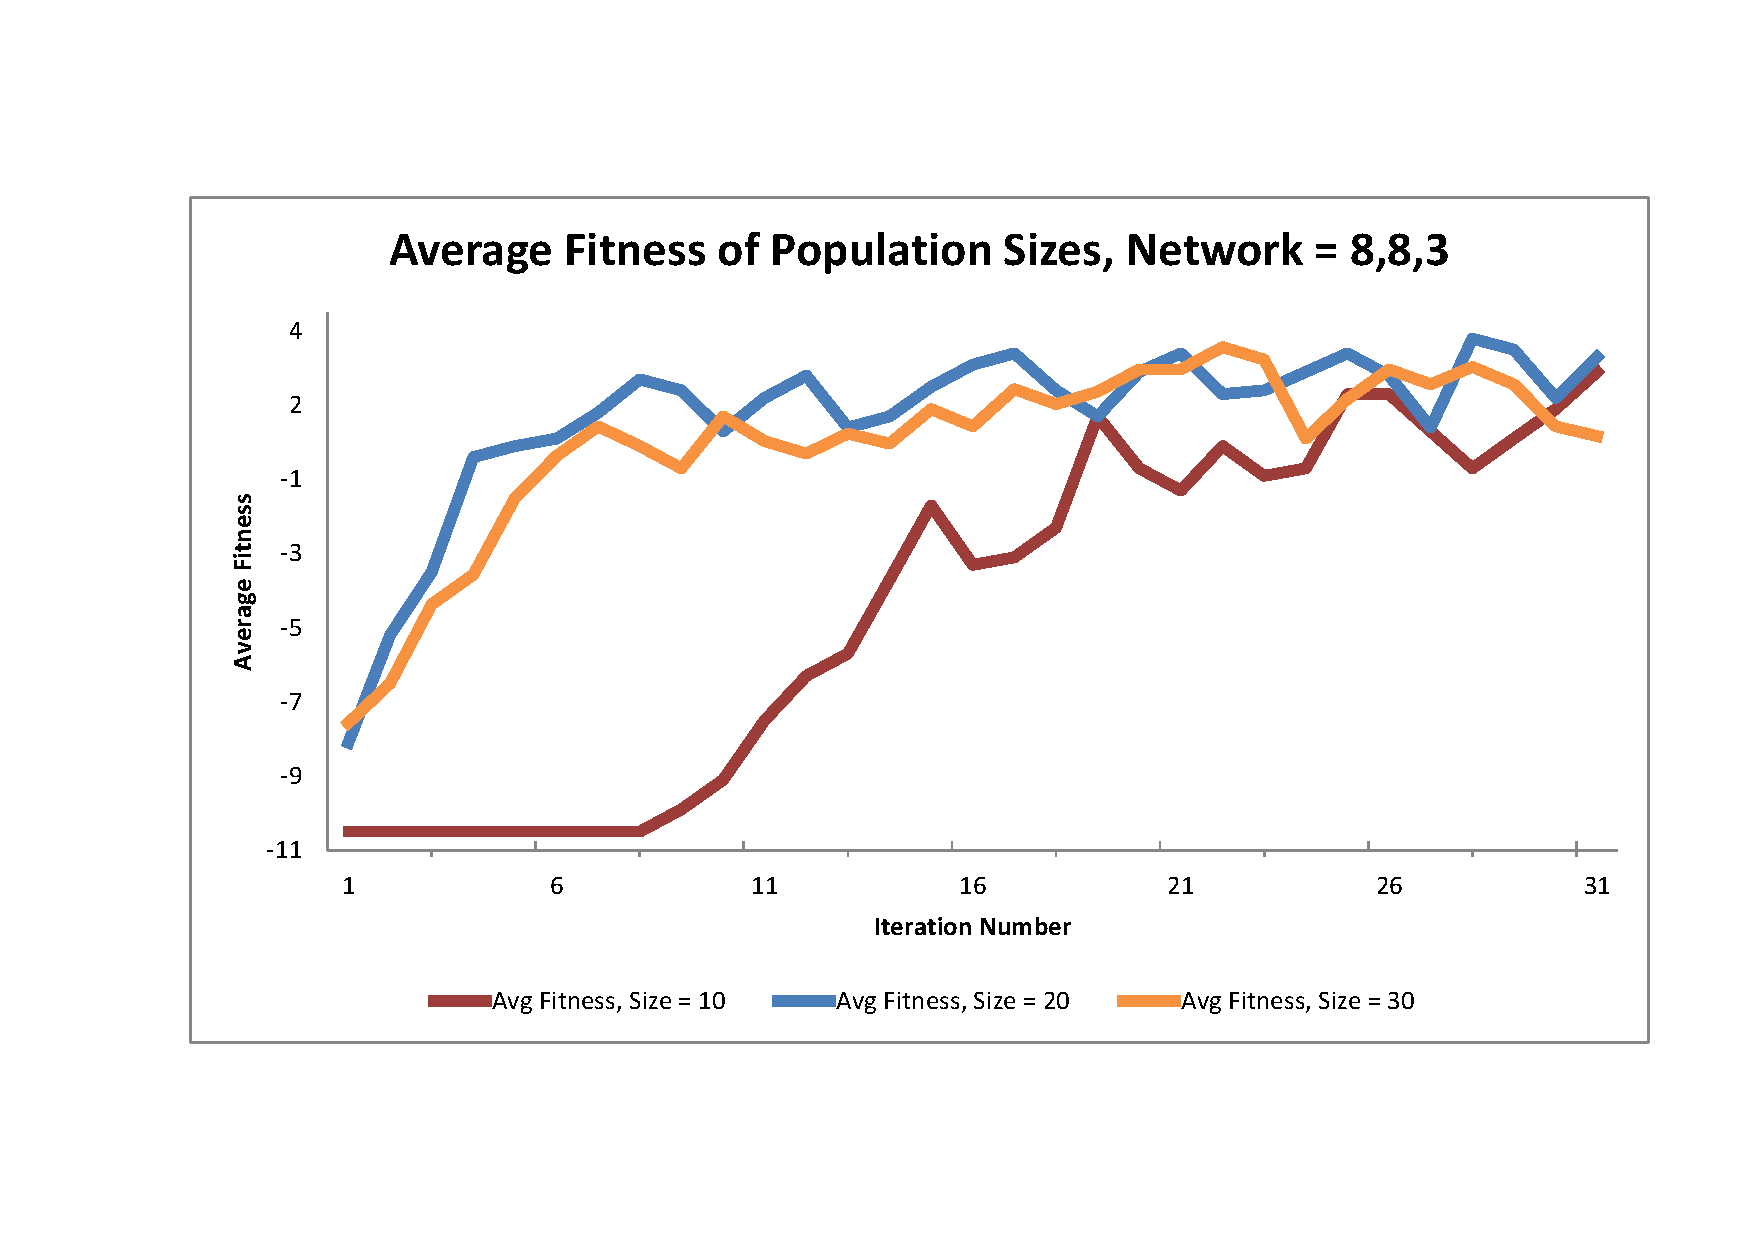
\includegraphics[width=1.0\columnwidth]{fig_GA_AverageFitness}}
\caption{Graph showing the progression of Average Fitness of population of size $10$, $20$ and $30$, respectively: NN configuration is $8,8,3$}
\label{fig:AverageFitness}
\end{figure}
\item Population Size - We are also interested in finding out the rate of convergence of the Genetic Algorithm, as well as its dependency on the population size. Generally a larger population size is preferred, since the high number of chromosomes provide a bigger search space for the algorithm to find a fit individual in. But this leads to a lot of overhead on the system to process individuals introduced on each iteration in the larger population. To assess this parameter, we look at a comparative Figure \ref{fig:AverageFitness} showing the progression of average fitness of the populations of sizes $10$, $20$ and $30$. The population with size 10 seems to be too small and has slow convergence to the other two populations. The other two populations are very close in average performance and hence a smaller and more efficient population size is selected. 
\begin{figure}[htp]
\centerline{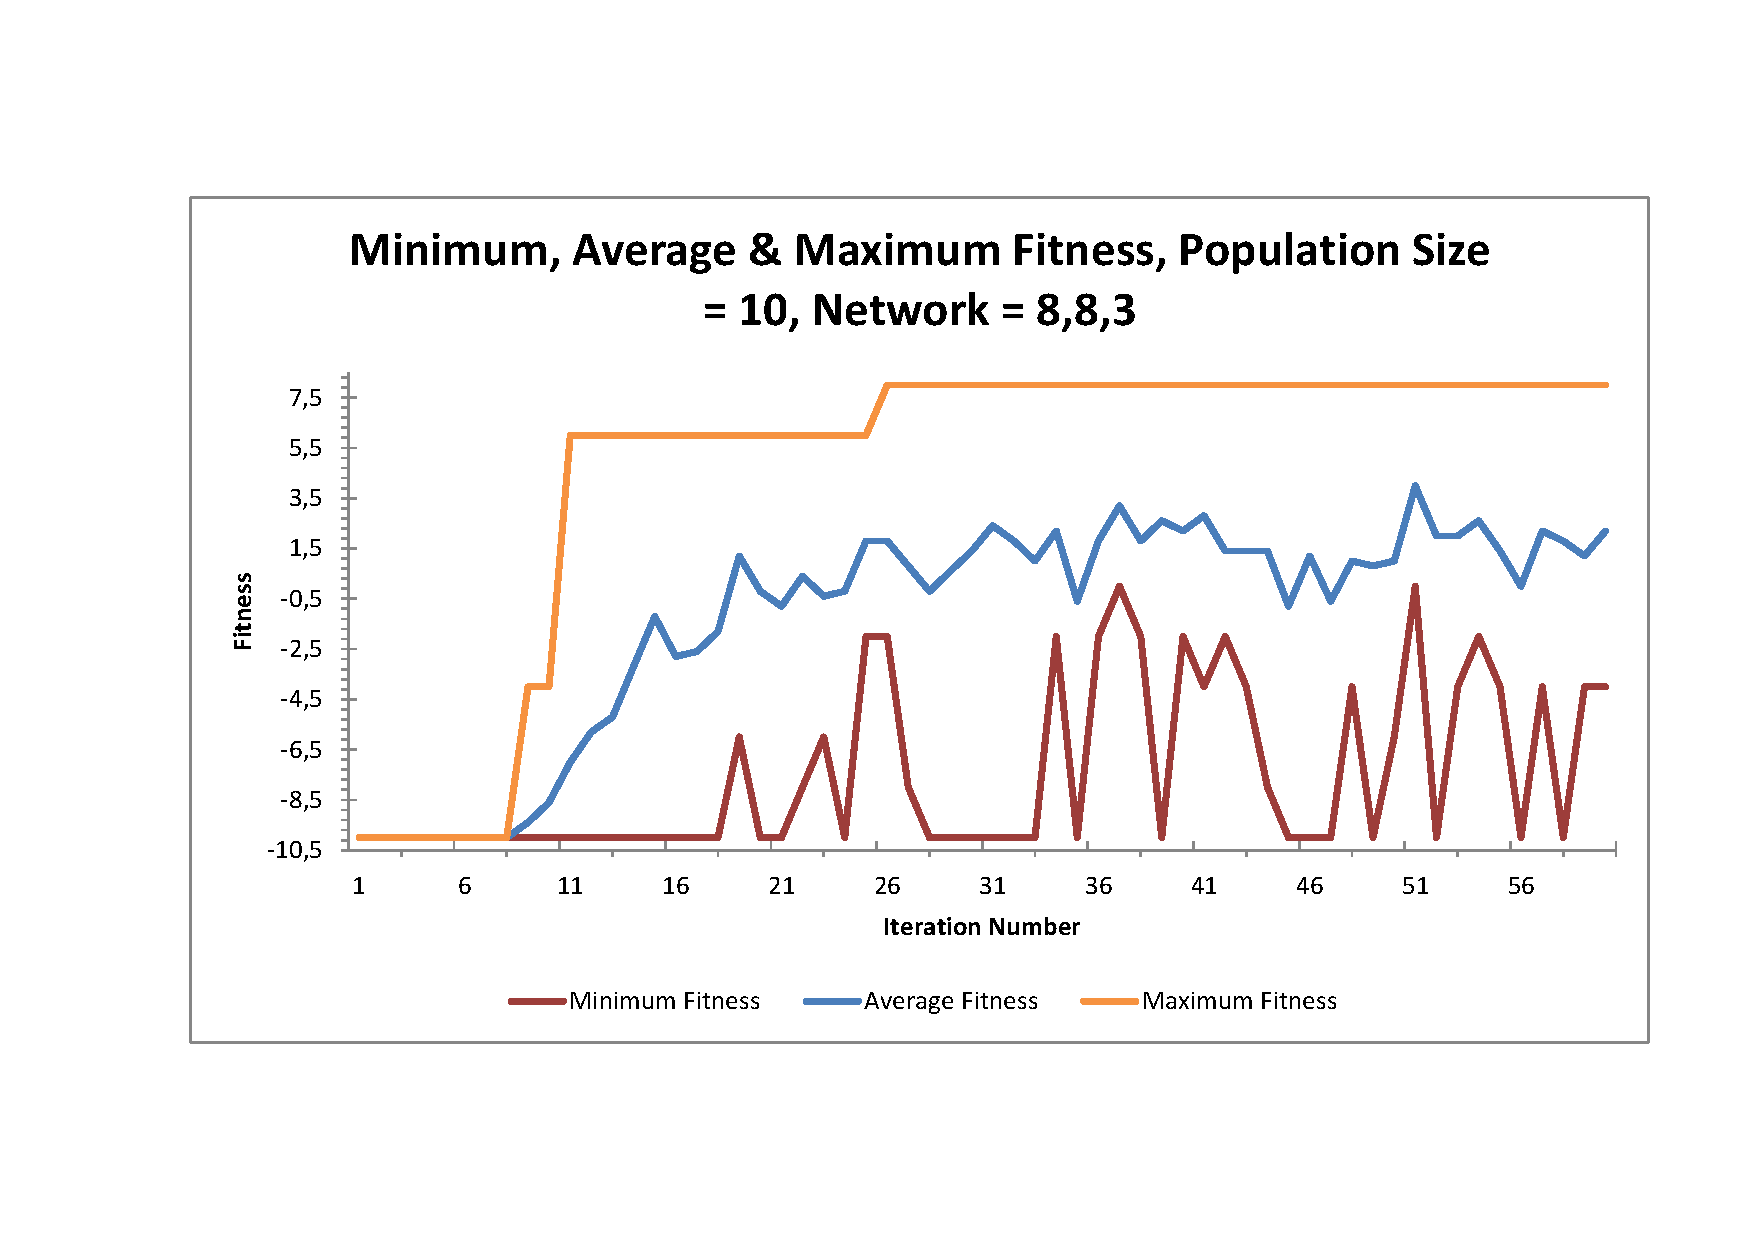
\includegraphics[width=1.0\columnwidth]{fig_GA_Fitness_MinAvgMax}}
\caption{Graph showing the minimum, average and maximum fitness of population of size $10$, NN configuration is $8,8,3$}
\label{fig:minAvgMaxFitness}
\end{figure}
\item Fitness Spread - In a genetic algorithm, the reproduction and discard rules are used to introduce new individuals to the population that can spread the solution in a much broader spectrum. This counters the problems provided by other computation intelligence algorithms to get stuck in local minima. A way to test the spread of the population is by graphing the minimum, average and maximum fitness of a population (size = $10$), as shown in Figure \ref{fig:minAvgMaxFitness}. A large distance between the minimum and maximum fitness points to the conclusion that the population is taking care of introducing diverse individuals.
\end{enumerate}

%%%
\begin{figure}[htp]
\centerline{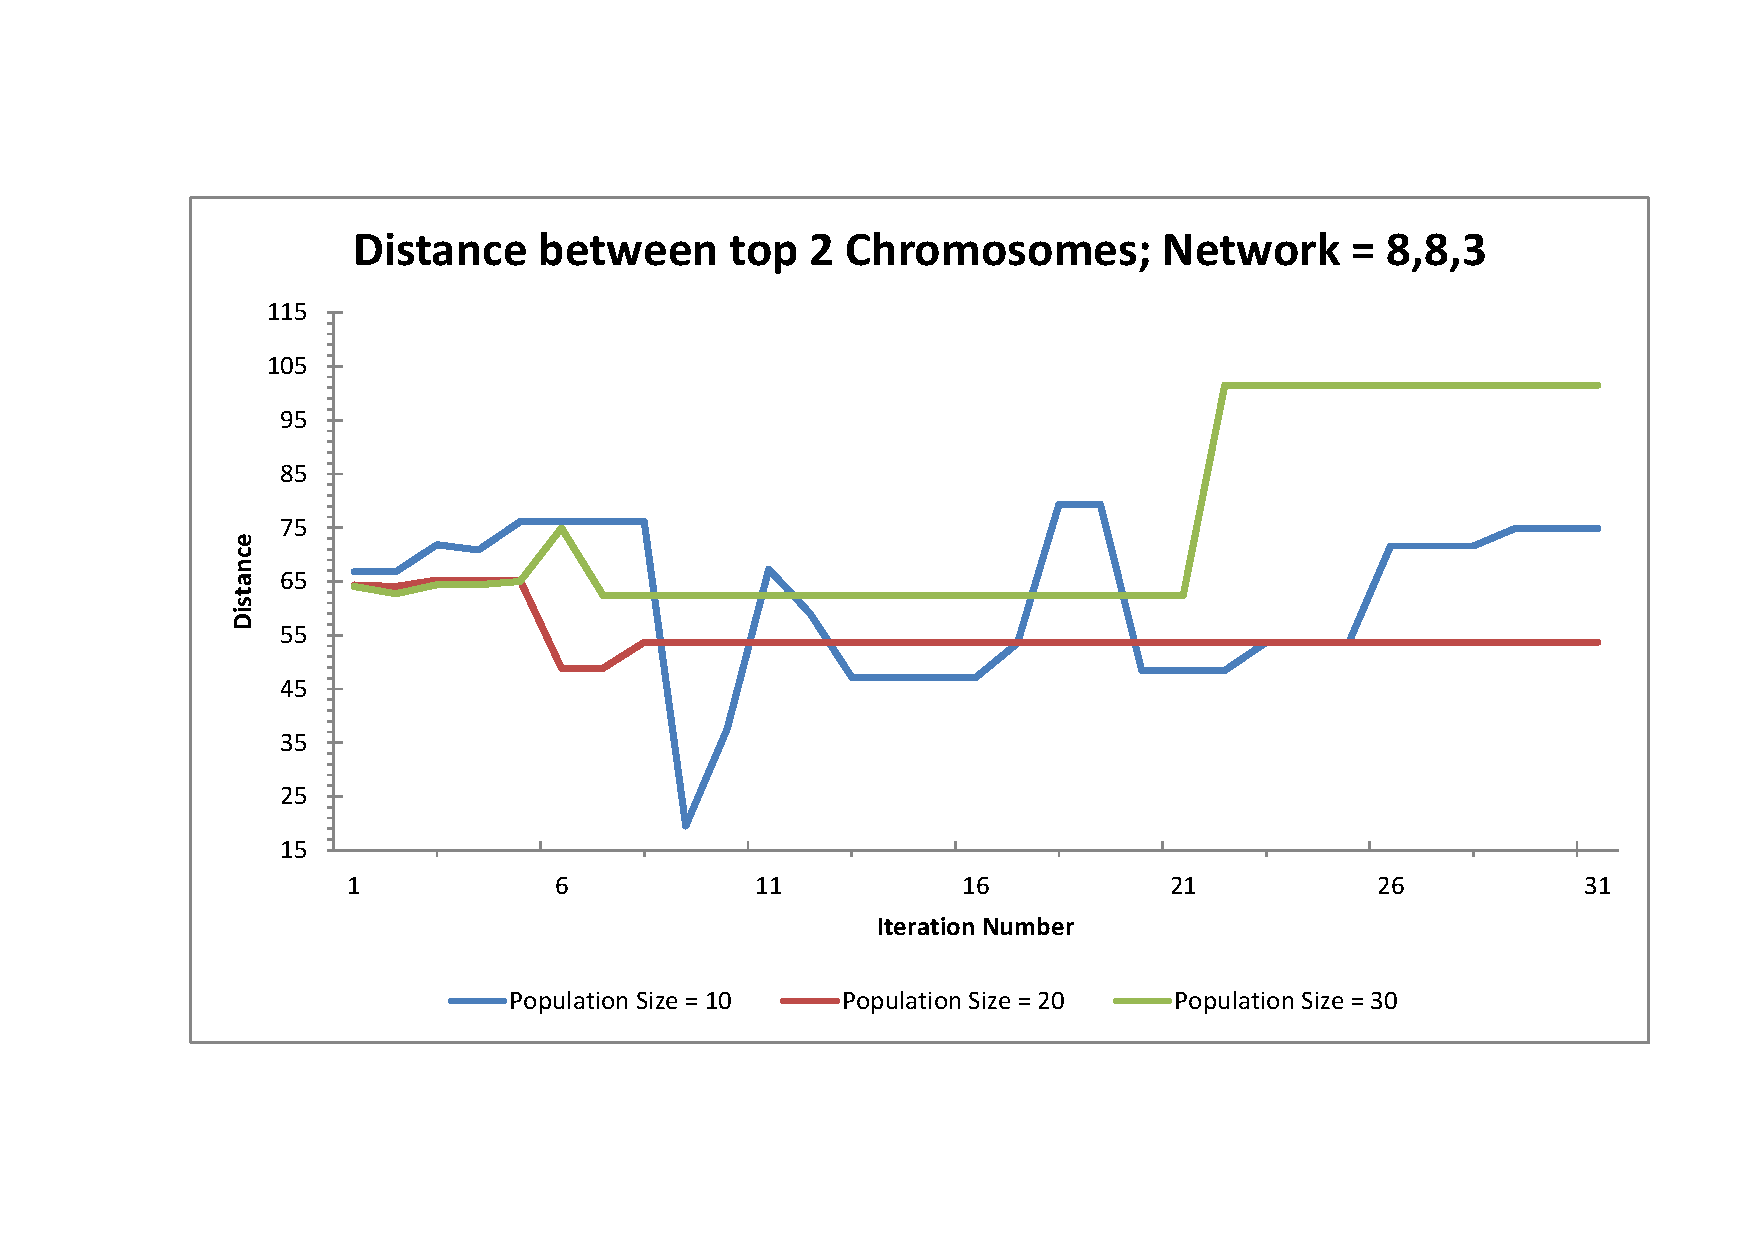
\includegraphics[width=1.0\columnwidth]{fig_GA_Speciation_Top2}}
\caption{Graph of Specie difference between the top two chromosomes}
\label{fig:specieTop2}
\end{figure}
\begin{figure}[htp]
\centerline{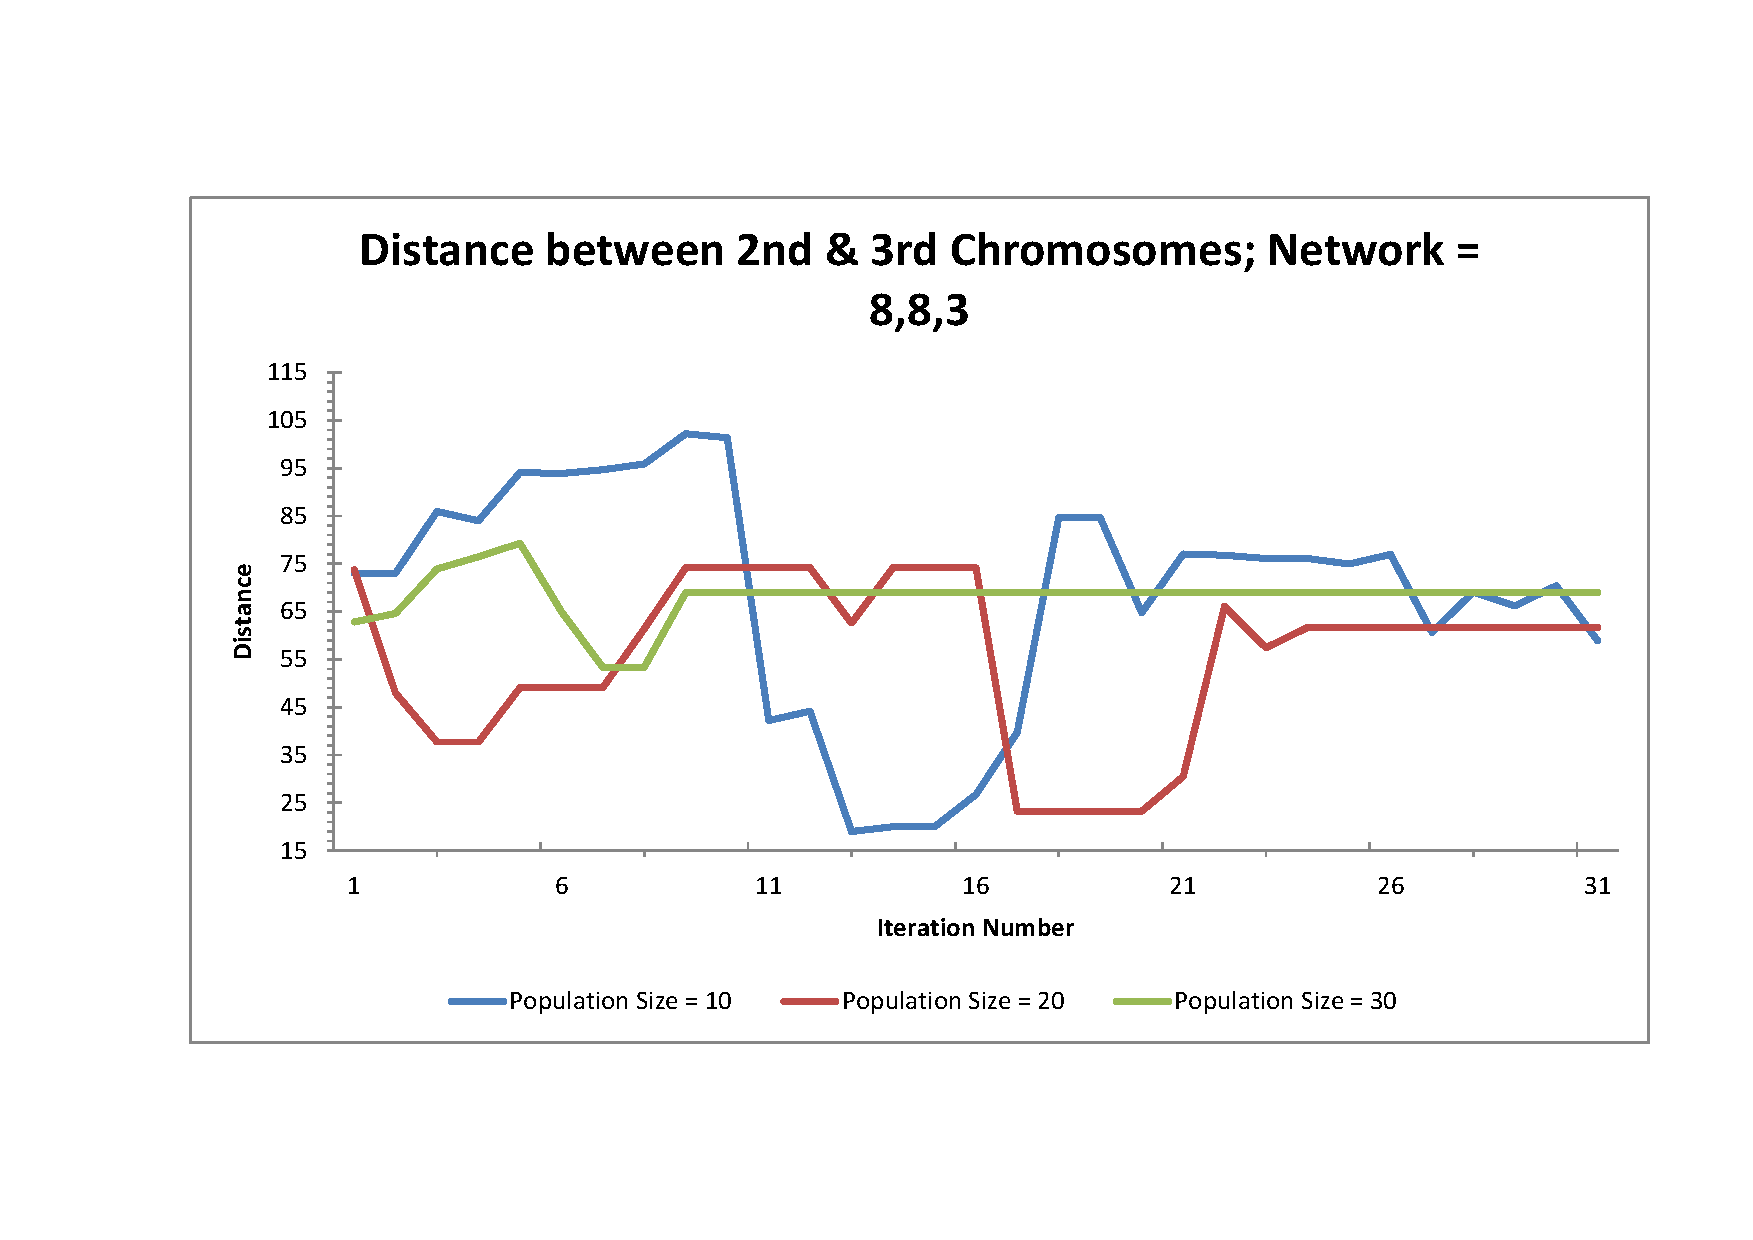
\includegraphics[width=1.0\columnwidth]{fig_GA_Speciation_next2}}
\caption{Graph of Specie difference between $2^{nd}$ and $3^{rd}$ ranked chromosomes}
\label{fig:specieNext2}
\end{figure}

%-------------------------------------------------------------------------------------------------------------------------------------------------
\subsection{Discussion}
According to our tests with the network structure and the population size, the best solution for our one versus one approach is a network structure of 8,8,3 and a population size of $20$. Although the bigger network also evolved well, in terms of performance we clearly have to choose the smaller one.
According to the figure \ref{fig:AverageFitness}, the population size of $20$, roughly scores as good as the population size of $30$. When we take the fact, that a smaller population size will evolve $\frac{1}{3}$ faster, into account, we have to chose a population size of $20$.

If we measure the cumulative distance between each gene of the top two candidates in the populations which is depicted in Figure \ref{fig:specieTop2}, we can see that the larger populations in genetic evolution hamper the evolving chances because of higher preservation of the top candidates. This can be attributes to the elite selection methodology we have employed that gives increasingly higher probability to the $1^{st}$ and $2^{nd}$ chromosomes to be selected for parenting.
This pattern becomes much more varied if we calculate the distance between the $2^{nd}$ and $3^{rd}$ chromosomes (Figure \ref{fig:specieNext2}), which depicts the higher chances for the chromosomes on those positions to be mutated.
%%%